\section{Sharding}
\label{sec:sharding}

The next improvement to the OR-Set is partitioning, or sharding, a replica into
many disjunctive subsets which can be stored individually on different machines.
Each replicated set can reside in a cluster, as illustrated in
Figure~\ref{fig:sharding_meaning}. Here Replica~1 is sharded in 3 subsets,
Replica~2 is sharded in 2 subsets, while Replica~3 is stored entirely on one
machine. This OR-Set data type where each replica set is sharded into subsets
will be referred to as \textbf{Sharded OR-Set} (\textbf{SOR-Set}).

\begin{figure}[b]
  \centering
  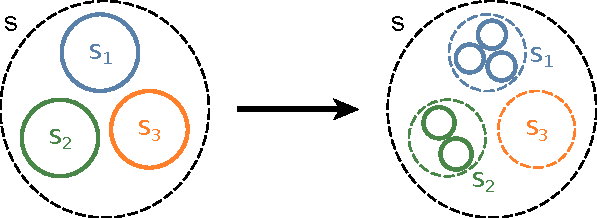
\includegraphics[width=0.6\linewidth]{sharding-meaning}
  \caption{Sharding of OR-Sets}
  \label{fig:sharding_meaning}
\end{figure}

In order to coordinate incoming requests for each of the replicated set, a
client entity should be used to forward the usual $\textit{add}(e)$,
$\textit{remove}(e)$, and $\textit{lookup}(e)$ operations to the corresponding
subset. For this purpose, the client can employ any partitioning function, such
as a hash function with uniform distribution, which maps each element $e$ to a
shard. The client is also responsible for initiating the \textit{merge}
operation between two clusters to pull the updates from all shards in the remote
cluster and distribute them according to the same hash function to the shards in
the local cluster.

\begin{algorithm}[t]
\small{
	\floatname{algorithm}{Specification}
	\caption{SOR-Set with delta-based synchronization}
 	\label{alg:sor_set}                       

 	\begin{algorithmic}[1]
      \State \Payload $A_{i}^{j} = \varnothing, R_{i}^{j} = \varnothing, T_{i}^{j} = [\,][\,], \forall j \in \{1,\ldots,|rc_{i}|\}$
      \State \textcolor{gray}{\Comment{$rc_{i}$ - Replica cluster $i$; $rs_{i}^{j}$ - Replica shard $j$ of $rc_{i}$}}

 	  \State \Query $lookup_{i}(e) : \text{boolean}$
 	  \State \hspace{\algorithmicindent} \Let $j = hash_{i}(e)$
 	  \State \hspace{\algorithmicindent} \Return $\exists (e, t, rc, rs) \in A_{i}^{j} \land \nexists (e, t, rc, rs, t', rc', rs') \in R_{i}^{j}$

 	  \State \Update $add_{i}(e)$
 	  \State \hspace{\algorithmicindent} \Let $j = hash_{i}(e)$
 	  \State \hspace{\algorithmicindent} \Let $rc = rc_{i}$
 	  \State \hspace{\algorithmicindent} \Let $rs = rs_{i}^{j}$
 	  \State \hspace{\algorithmicindent} \Let $t = T_{i}^{j}[rc][rs] + 1$
 	  \State \hspace{\algorithmicindent} $A_{i}^{j} \coloneqq A_{i}^{j} \cup \{(e, t, rc, rs)\}$
 	  \State \hspace{\algorithmicindent} $T_{i}^{j}[rc][rs] \coloneqq t$

 	  \State \Update $remove_{i}(e)$
 	  \State \hspace{\algorithmicindent} \Pre $lookup_{i}(e)$
 	  \State \hspace{\algorithmicindent} \Let $j = hash_{i}(e)$
 	  \State \hspace{\algorithmicindent} \Let $rc' = rc_{i}$
 	  \State \hspace{\algorithmicindent} \Let $rs' = rs_{i}^{j}$
 	  \State \hspace{\algorithmicindent} \Let $t' = T_{i}^{j}[rc'][rs'] + 1$
 	  \State \hspace{\algorithmicindent} $R_{i}^{j} \coloneqq R_{i}^{j} \cup \{(e, t, rc, rs, t', rc', rs') \mid \exists (e, t, rc, rs) \in A_{i}^{j}\}$
 	  \State \hspace{\algorithmicindent} $T_{i}^{j}[rc'][rs'] \coloneqq t'$
 	  
 	  \State \Compare $(rc_{x}, rc_{y}) : \text{boolean}$
 	  \State \hspace{\algorithmicindent} \Let $\tilde{T}_{x} = version(rc_{x})$
 	  \State \hspace{\algorithmicindent} \Let $\tilde{T}_{y} = version(rc_{y})$
 	  \State \hspace{\algorithmicindent} \Return $(\bigcup_{j} A_{x}^{j} \subseteq \bigcup_{k} A_{y}^{k}) \land (\bigcup_{j} R_{x}^{j} \subseteq \bigcup_{k} R_{y}^{k}) \land (\tilde{T}_{x} \leq \tilde{T}_{y})$
 	  \State \hfill $\forall j \in \{1,\ldots,|rc_{x}|\}; \forall k \in \{1,\ldots,|rc_{y}|\}$
 	  
 	  \State \Merge $(rc_{x}, rc_{y}) : \text{payload}$
 	  \State \hspace{\algorithmicindent} \Let $\tilde{T}_{x} = version(rc_{x})$
 	  \State \hspace{\algorithmicindent} \Let $\tilde{T}_{y} = version(rc_{y})$
 	  \State \hspace{\algorithmicindent} $\forall j \in \{1,\ldots,|rc_{y}|\}$
      \State \hspace{\algorithmicindent} \hspace{\algorithmicindent} \Let $A' = \{(e, t, rc, rs) \in A_{y}^{j} \mid \tilde{T}_{x}[rc][rs] < t\}$
      \State \hspace{\algorithmicindent} \hspace{\algorithmicindent} \Let $R' = \begin{aligned}[t]
                                                                                  & \{(e, t, rc, rs, t', rc', rs') \in R_{y}^{j} \\[-2pt]
                                                                                  & \mid \tilde{T}_{x}[rc'][rs'] < t'\}
                                                                                \end{aligned}$
      \State \hspace{\algorithmicindent} $\forall j \in \{1,\ldots,|rc_{x}|\}$
      \State \hspace{\algorithmicindent} \hspace{\algorithmicindent} \Let $Z.A_{x}^{j} = A_{x}^{j} \cup \{(e, t, rc, rs) \in A' \mid j = hash_{x}(e)\}$
      \State \hspace{\algorithmicindent} \hspace{\algorithmicindent} \Let $Z.R_{x}^{j} = \begin{aligned}[t]
                                                                                          & R_{x}^{j} \cup \{(e, t, rc, rs, t', rc', rs') \in R' \\[-2pt]
                                                                                          & \mid j = hash_{x}(e)\}
                                                                                         \end{aligned}$
      \State \hspace{\algorithmicindent} \hspace{\algorithmicindent} \Let $Z.T_{x}^{j} = max(T_{x}^{j}, \tilde{T}_{y})$
      \State \hspace{\algorithmicindent} \Return $Z$
	\end{algorithmic}
 }
\end{algorithm}

Specification~\ref{alg:sor_set} synthesizes the usual state-based operations.
Each replica $i$ of the set is stored in a \textit{replica cluster} $rc_{i}$.
Inside the cluster $rc_{i}$, the set is partitioned into $|rc_{i}|$ subsets,
called \textit{replica shard}s $rs_{i}^{j}$. Therefore, any shard is uniquely
identified by the pair of identifiers $(rc, rs)$. Based on this observation,
instead of using a timestamp vector to keep track of the latest versions for the
replicas as in the previous section, a vector of timestamp vectors $T$ is
used. $T$ has as many components as there are clusters, while $T[rc_{i}]$ has
$|rc_{i}|$ components, one for each shard. Like before, each cell $T[rc][rs]$
stores the latest version of the logical clock of the shard $(rc, rs)$. Each
shard has its own $T$. Since when adding or removing an element from the source
replica, it will be added or, respectively, removed from only one shard $(rc,
rs)$, i.e. the one computed by the hash function, each update can be uniquely
tagged with the tuple $(t, rc, rs)$, where $t$ is the timestamp generated at
$(rc, rs)$.

Returning to the specification, the payload is also distributed: $A_{i}^{j}$,
$R_{i}^{j}$, and $T_{i}^{j}$ are, respectively, the set of added and removed
elements and the vector of timestamps for shard $rs_{i}^{j}$. The set operations
follow the same principle as before. Merging the state of a remote replica from
cluster $rc_{y}$ into the local state in cluster $rc_{x}$ is also similar. We
just need to compute a minimum version $\tilde{T}_{x}$ first for the whole
cluster by combining the information from all $T_{x}^{j}$ using
$version(rc_{x})$ defined as:
% \small
\begin{align*}
\tilde{T}_{x}[rc][rs] = \begin{cases}
                            max (\bigcup_{j \in \{1,\ldots,|rc_{x}|\}} T_{x}^{j}[rc][rs]) & \text{if } rc = rc_{x}, \\
                            min (\bigcup_{j \in \{1,\ldots,|rc_{x}|\}} T_{x}^{j}[rc][rs]) & \text{otherwise}
                        \end{cases}
\\
\hfill \forall rc = rc_{i}, i \in \{1,\ldots,N\}; \forall rs = rs_{i}^{j}, j \in \{1,\ldots,|rc_{i}|\}.
\end{align*}
% \normalsize

We set the minimum from all $T_{x}^{j}$ component-wise, except for
$\tilde{T}_{x}[rc_{x}]$, where we choose the maximum instead since each shard in
$rc_{x}$ increments its own counter only. We do the same for cluster $rc_{y}$.

Some important observations are worth mentioning. First, the \textit{merge}
operation remains unobtrusive like for all CRDTs: clients can issue requests to
the set while the operation progresses in the background. Since the minimum
version $\tilde{T}_{y}$ is computed first, the remote cluster $rc_{y}$ can
meanwhile process any subsequent updates. They will be pulled with the next
merge. Analogously, because at the end each $T_{x}^{j}$ is updated to the
maximum between the current one and the remote one component-wise, the local
cluster can in this time process any incoming client requests. Therefore, both
sets can be updated while the synchronization takes place. 

Second, this algorithm is resilient to shard failures in both local and remote
clusters. An unreachable shard in the local cluster leads to a potential bigger
$\tilde{T}_{x}$ except for $\tilde{T}_{x}[rc_{x}]$. This means that not all
updates will be fetched. As soon as the failed shard restores, its lagging
timestamp will lead to a smaller $\tilde{T}_{x}$ and the next merge will thus
include the missing updates plus some of the already fetched ones. For the
remote cluster, an unreachable shard has the same consequence: $T_{x}^{j}
\coloneqq max(T_{x}^{j}, \tilde{T}_{y})$ will set smaller values in
$T_{x}^{j}[rc_{y}]$ and missed updates will be fetched with the next merge after
the shard restores.

\begin{proof}[Proof that sharding maintains the CRDT properties]
Consider a replica state as $s_{i} = (A_{i}, R_{i}, \tilde{T}_{i})$, where
$A_{i} = \bigcup_{j \in \{1,\ldots,|rc_{i}|\}} A_{i}^{j}$ and $R_{i} =
\bigcup_{j \in \{1,\ldots,|rc_{i}|\}} R_{i}^{j}$. Thus, a set is characterized
by the contributions of all its subsets. The partial order is then $(S,
\sqsubseteq)$, $\forall s_{i} \in S$ and $\sqsubseteq$ given by \textit{compare}
method. Update operations \textit{add} and \textit{remove} advance the state in
the partial order as they both add elements to the set and increase $\tilde{T}$.
\textit{Merge} computes the set union between $A_{x}$ and $A_{y}$ and between
$R_{x}$ and $R_{y}$, respectively. Also, because each $T_{x}^{j}$ is updated
with the maximum between $T_{x}^{j}$ and $\tilde{T}_{y}$, the newly obtained
$\tilde{T}_{x}$ will be the maximum between $\tilde{T}_{x}$ and $\tilde{T}_{y}$.
Therefore \textit{merge} computes the LUB.
\end{proof}